\documentclass{elsarticle}
\usepackage[utf8]{inputenc}
\usepackage{kpfonts}
\usepackage[labelfont=bf]{caption}
\usepackage{graphicx}
\usepackage{subfig}
\usepackage{stmaryrd}
\captionsetup[figure]{name=Fig. ,labelsep=period}

\newcommand{\choice}{|}
\newdefinition{definition}{Definition}
\newtheorem{notation}{Notation}
\newtheorem{theorem}{Theorem}
\newdefinition{example}{Example}
\newdefinition{running_example}{Running example}

\begin{document}

% title page
\begin{frontmatter}
\title{Formal Biochemical Space Language}

\author{\normalsize
Matej Troják, David Šafránek and Františka Romanovská}
\address{Faculty of Informatics, Masaryk University\\
Brno, Czech Republic
}

\begin{abstract}
Biochemical Space (BCS) has been introduced as a formal notation for reaction networks of biological processes by translating to Kappa language. In this paper, we define our language directly to employ own syntactic and semantic abstractions which increase expressiveness and compactness of the language.
\end{abstract}

\begin{keyword}
rule-based modelling
\end{keyword}

\end{frontmatter}

\section{Introduction}

Why BCS with its own semantics

\begin{figure}[!h]
\begin{center}
\framebox{
{\small
\begin{tabular}{ l | l }
 ENTITY ID: & KaiC\\
 STATES:\\
 LOCATIONS: & cyt\\
 COMPOSITION: & S $|$ T\\
 ENTITY NAME: & circadian clock protein kinase KaiC\\
 CLASSIFICATION: & enzyme\\
 DESCRIPTION: & Monomer component representing a core component\\
 & of the circadian clock system.\\
 LINKS: & uniprot::Q79PF4, cyanobase::Synpcc7942\_1216\\
 ORGANISM: & Synechococcus elongatus PCC 7942
\end{tabular}}
}
\end{center}
\caption{Example of an entity -- complete information given for a structure entity.}\label{ex:structureent}
\end{figure}

\begin{itemize}
	\item show example of a BCS record with all the metadata -- it shows why BCS is useful
	\begin{itemize}
		\item a record with full information, mention it comes from ecyano where it is being used, some blabla about ecyano would be suitable
	\end{itemize}
	\item show clock in BCSL and Kappa (quite huge, how to show briefly?) -- it prooves BCSL's compactness
	\begin{itemize}
		\item maybe just some important rule to compare (phosphorylation for example)
	\end{itemize}
	\item semantical examples -- explain our complex agents are not really complexes with bonds (such as in Kappa). It has more abstract meaning of \emph{coexistence}, ie. not just a complex with bonds but all other kinds of shared existence. Example: enzymatic reaction, usually A + E $\Rightarrow$ B + E, however, we dont like this kind of expressions, its not clear what is actually happening. Another example: A + C + E $\Rightarrow$ B + D + E. This example shows it really isnt clear from biological point of view. Thats why we prohibit this and the coexistence of objects must be first declared as a complex agent. 
	\item Another example should be about atomic agents. One (an amino acid?) might be used in a complex and also structural agent. That could not happen in Kappa, it would be agent and a site -- quite difference. This should show huge advantage of structural agents which Kappa lacks. 
	\item another important thing is some kind of \emph{encapsulation} -- in Kappa, when you write a rule where an agent is being changed (anyhow), its possible to express it regardless the bond, ie. it might be free or bonded. This is impossible in BCSL since we have special agents for complexes. It follows we employ a kind of encapsulation: a rule changing atomic agent does not change it inside a partial composition (structural agent) or full composition (complex agent)
\end{itemize}

\section{Rule-based basics (intro)}

In our last paper~\cite{Ded201627}, we defined semantics of Biochemical Space Language (BCSL) via translating to a similar language called Kappa~\cite{Kappa}. However, we realised this approach is not very beneficial since we are not fully using the expressive power of our language this way. The thing is Kappa operates purely on expressions. We want to promote our language to a higher level when it operates on objects in multisets. By translating to Kappa we loose such abstraction. 

The reason for this kind of abstraction is the way how we see the biological models. We represent model $\mathcal{M}$ as set of rules and an initial solution of interacting entities. We understand solution as a mixture of individual objects which are randomly distributed (see Fig.~\ref{solutions:fig}a). Therefore, we cannot assign them any order and we do not see them as expressions but rather as multisets. For us, this representation of solution is the closest to the reality.

\begin{figure}
\begin{center}
\subfloat[]{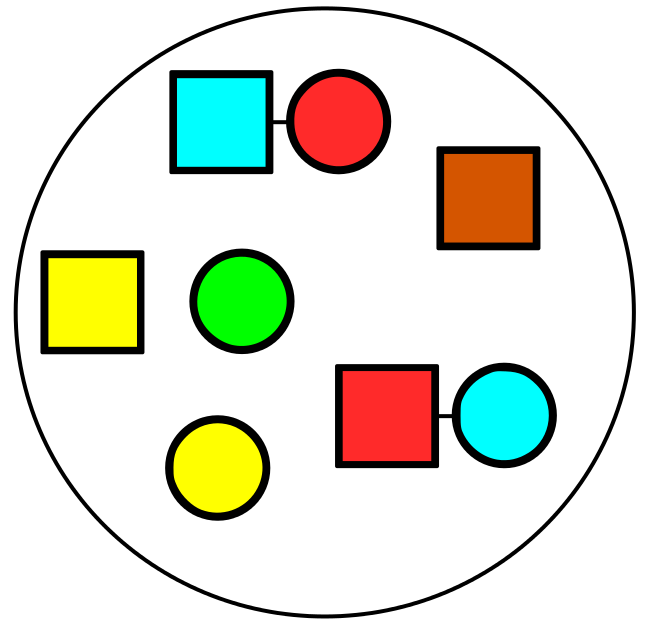
\includegraphics[scale=0.23]{solution_first}\label{sol:s1}}
\hspace*{1cm}
\subfloat[]{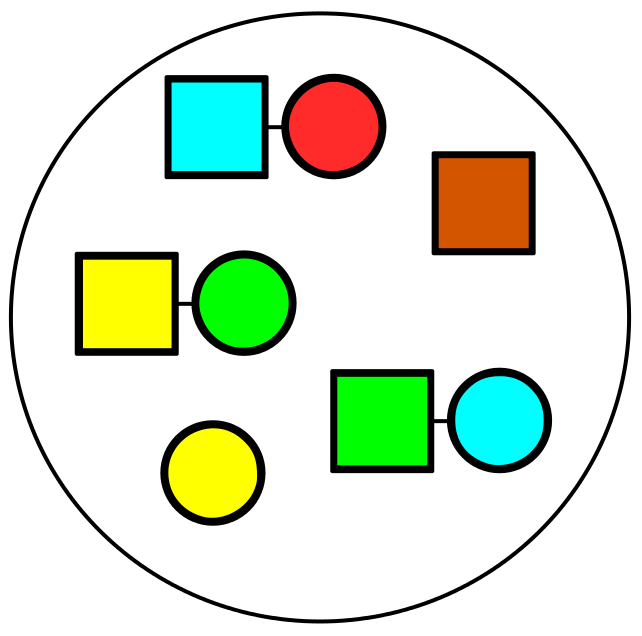
\includegraphics[scale=0.23]{solution_second}\label{sol:s2}}
\caption{\textbf{Examples of solutions}. \textbf{(a)} An example of graphical representation of a solution. \textbf{(b)} Updated solution after rules from Fig.~\ref{rules:fig} were applied. The first rule \textit{(a)} was applied on the yellow $\square$ and green $\bigcirc$ and produced yellow-green complex $\square$--$\bigcirc$. Note there are more options how the rule could be mapped -- each combination of free $\square$ and $\bigcirc$. The second rule \textit{(b)} was applied on red-cyan complex $\square$--$\bigcirc$ where the color of $\square$ was changed from red to green. The third rule \textit{(c)} couldn't be applied because there is no such complex with yellow $\bigcirc$. }
\label{solutions:fig}
\end{center}
\end{figure}

On the other hand, the rules are expressions which describe behaviour of groups of objects. A rule has form of a chemical reaction, where substrates and products take place. The difference is that reaction only operates on particular objects. Therefore, a reaction can be seen as a special case of rule (see Fig.~\ref{rules:fig}), where the groups contain exactly one element.

The rule can be mapped on a solution. Then, if it is mapped, it can be applied and a new solution is produced. The mapping is not always successful (see Fig.~\ref{solutions:fig}, application of rule \textit{c}). By repeating map-apply action, we obtain a \textit{Labelled transition system} $\mathcal{L}$.

\begin{definition}\label{lts}
\textit{Labelled transition system} (LTS) $\mathcal{L}$ is a tuple $(S, A, \Delta, s_0)$ where:
\begin{itemize}
	\item $S$ is a (potentially infinite) set of states (solutions)
	\item $A$ is a set of labels (reactions)
	\item $\Delta \subseteq S \times A \times S$ is a transition relation (the map-apply action)
	\item $s_0 \in S$ is the initial state (initial solution)
\end{itemize}
\end{definition}

\begin{figure}[!h]
\begin{center}
\begin{minipage}[l]{0.1\textwidth}
    \textbf{(a)}
  \end{minipage}
  \begin{minipage}[r]{0.6\textwidth}
    {\hspace*{0.8cm}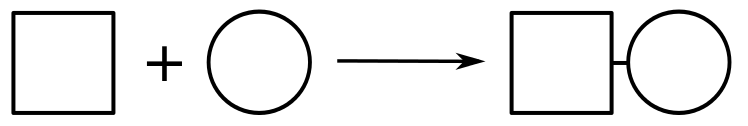
\includegraphics[scale=0.2]{rule_complex}}
\end{minipage}

\begin{minipage}[l]{0.1\textwidth}
    \textbf{(b)}
  \end{minipage}
  \begin{minipage}[r]{0.6\textwidth}
    {\hspace*{1.35cm}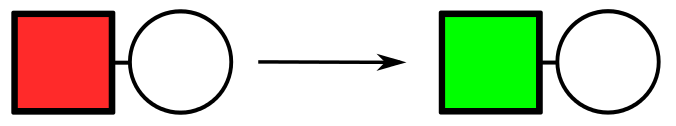
\includegraphics[scale=0.2]{rule_change}}
\end{minipage}

\begin{minipage}[l]{0.1\textwidth}
    \textbf{(c)}
  \end{minipage}
  \begin{minipage}[r]{0.6\textwidth}
    {\hspace*{1.3cm}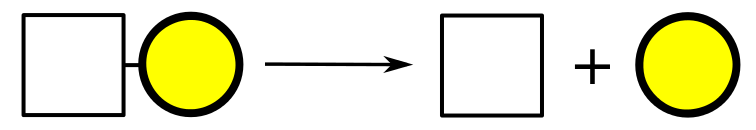
\includegraphics[scale=0.2]{rule_diss}}
\end{minipage}
\caption{\textbf{Examples of rules}. Rule \textbf{(a)}: a $\square$ and a $\bigcirc$ can form a complex $\square$--$\bigcirc$ regardless their colors. Rule \textbf{(b)}: a $\square$ is allowed to change it's color from red to green only if it formed a complex with a $\bigcirc$ regardless it's color. Rule \textbf{(c)}: the rule can disassemble the complex only if the $\bigcirc$ is yellow.}
\label{rules:fig}
\end{center}
\end{figure}

The mapping of a rule on a solution can be seen as a particular moment, when the objects in the solution have just the conformation suitable for the rule and therefore the rule can be applied. However, since the distribution of objects is random, we can assume a sequence of objects needed for rule (if there are such objects) is always available.

Moreover, the mapping can be seen as assigning particular objects from the solution to objects on the left-hand-side of the rule. The rule application can be seen as changing the mapped objects to new objects according to the right-hand-side of the rule (i.e., particular objects are assigned to the right-hand-side). As a by-product, we obtain an instance of the rule -- a reaction (see Fig.~\ref{map-apply:fig}). This is how we construct the set of reactions $A$ in the LTS $\mathcal{L}$.

\begin{figure}
\begin{center}
\begin{minipage}[l]{0.1\textwidth}
    \textbf{(a)}
  \end{minipage}
  \begin{minipage}[r]{0.6\textwidth}
    {\hspace*{1.3cm}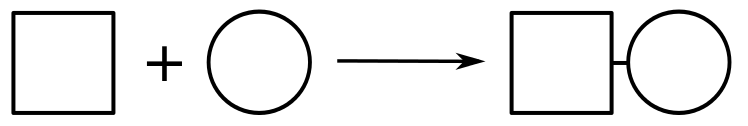
\includegraphics[scale=0.2]{rule_complex}}
\end{minipage}

\begin{minipage}[l]{0.1\textwidth}
    \textbf{(b)}
  \end{minipage}
  \begin{minipage}[r]{0.6\textwidth}
    {\hspace*{1.3cm}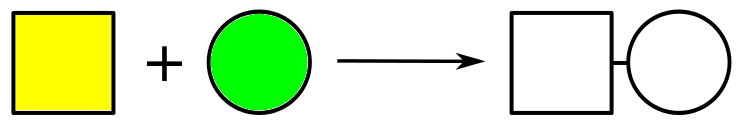
\includegraphics[scale=0.2]{rule_complex_mapped}}
\end{minipage}

\begin{minipage}[l]{0.1\textwidth}
    \textbf{(c)}
  \end{minipage}
  \begin{minipage}[r]{0.6\textwidth}
    {\hspace*{1.3cm}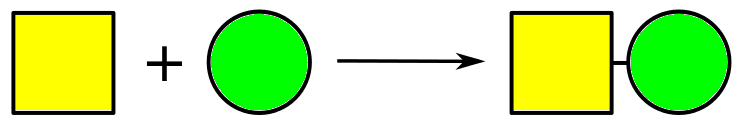
\includegraphics[scale=0.2]{rule_reaction}}
\end{minipage}
\caption{\textbf{Example of a map-apply action}. As a solution, we use solution \textit{(a)} from Fig.~\ref{solutions:fig}. \textbf{(a)} Rule can be mapped on a $\square$ and a $\bigcirc$ regardless their colors and form a complex $\square$--$\bigcirc$.  \textbf{(b)} Let's choose yellow $\square$ and green $\bigcirc$ from our solution. The rule was mapped on choosen objects and they were assigned to the left-hand-side of the rule. \textbf{(c)} The rule was applied and new object (yellow-green complex $\square$--$\bigcirc$) was created. We obtained the reaction describing the particular action which has just happened.}
\label{map-apply:fig}
\end{center}
\end{figure}

Since this kind of graphical representation is not very suitable for describing the processes and for transferring them.. ???, in next chapter(s) we define a formal language which is built on principles described in this chapter.

%%%%%%%%%%%%%%%%%%%%%%%%%%%%%%%%%%%%%%%%%%%%%%%%%%%%%%%%%%%%%%%%%%%%%%%%%%%%%%%%%%%%%
% multisets

\section{Background}
\subsection{Multiset definitions}

Let $\mathtt{E}$ be a set. A multiset $\mathrm{M}$ can be seen as a mapping $\mathtt{E} \rightarrow \mathbb{N}$ where $\mathbb{N}$ is set of natural numbers. Let $\mathscr{M}(\mathtt{E})$ be the set of all the finite multisets on $\mathtt{E}$, i.e. the multisets $\mathrm{M}$ such that their support $\{ x \in \mathtt{E} | \mathrm{M}(x) \neq 0 \}$ is finite.

The empty multiset \{ \} is the multiset such that \{ \}(x) = 0, for all $x \in \mathtt{E}$. A set is a particular cas of multiset such that $\mathrm{M}(x)$ is 0 or 1. Usually multisets are denoted by lists $\{ x_1, \ldots, x_m \}$ with a straightforward interpretation. If $\mathrm{M}$ is a multiset, $x \in \mathrm{M}$ means $\mathrm{M}(x) > 0$.

\begin{definition}
\emph{Equivalence of multisets.}

\noindent A multiset $\mathrm{M}$ is equivalent to a multiset $\mathrm{N}$ ($\mathrm{M} \equiv \mathrm{N}$) iff $\forall x \in \mathtt{E}: \mathrm{M}(x) = \mathrm{N}(x)$.
\end{definition}

\begin{definition}
\emph{Sum of multisets.}

\noindent The sum of two multisets $\mathrm{M}$ and $\mathrm{N}$ is the multiset $\mathrm{M}$ + $\mathrm{N}$ such that $\mathrm{M}$ + $\mathrm{N}(x)$ = $\mathrm{M}(x)$ + $\mathrm{N}(x)$.
\end{definition}

\begin{definition}
\emph{Inclusion of multisets.}

\noindent A multiset $\mathrm{M}$ is included in a multiset $\mathrm{N}$ ($\mathrm{M} \subseteq \mathrm{N}$) iff $\forall x \in \mathtt{E}: \mathrm{M}(x) \leq \mathrm{N}(x)$.

We say $\mathrm{M}$ `is a \emph{subset}' of $\mathrm{N}$ instead of `is a \emph{submultiset}'.
\end{definition}


\begin{definition}
\emph{Difference of multisets.}

\noindent If $\mathrm{M} \subseteq \mathrm{N}$, the difference $\mathrm{N}$ $\setminus$ $\mathrm{M}$ is defined by $\mathrm{N}$ $\setminus$ $\mathrm{M}(x)$ = $\mathrm{N}(x)$ $\setminus$ $\mathrm{M}(x)$.
\end{definition}

\noindent\rule{\textwidth}{1pt}

\begin{definition}
\emph{Concatenation of tuples.}

\noindent $X = (x_1, \ldots, x_n)$, $Y = (y_1, \ldots, y_m)$ be tuples, i.e. ordered sets (multisets). We define \emph{concatenation of tuples} $X \cdot Y$ as a tuple $X \cdot Y := (x_1, \ldots, x_n, y_1, \ldots, y_m)$.

Moreover, we extend the definition to concatenation of tuple $X$ with set of tuples $\{ Y_1, Y_2, \ldots, Y_n \}$ as following:

\begin{center}
$X \cdot \{ Y_1, Y_2, \ldots, Y_n \} := X \cdot Y_1 \cdot \{ Y_2, \ldots, Y_n \}$

$ X \cdot \emptyset := X $
\end{center}

\end{definition}

\begin{definition}
\emph{Appending an element to a tuple.}

Appending an element $x$ to a tuple $X = (x_1, \ldots, x_n)$, written $x \oplus X$, is a new tuple $Y = (x, x_1, \ldots, x_n)$

MORE PRECISE DEFINITION NEEDED !
\end{definition}

%%%%%%%%%%%%%%%%%%%%%%%%%%%%%%%%%%%%%%%%%%%%%%%%%%%%%%%%%%%%%%%%%%%%%%%%%%%%%%%%%%%%%
% BCSL

\section{Biochemical Space}

Biological background for mathematical model is provided by Biochemical Space. BCS is represented as a text file, that is human readable and visualised on website(!!cite). It contains two parts – set of entities and rules. BCS contains a hierarchy of entities ranging from small molecule through structures to large complex molecules. Rules are abstractly represented by chemical reactions defined over the set of entities. Because of tight coupling of an entity and a rule definitions with information from ontologies, annotation attributes are used.

Emphasis is put on well-defined and complete annotations – links to relevant existing ontologies for each rule and entity. Hypertext links to KEGG, ChEBI and CyanoBase are used at the moment, other databases and multiple link are supported. Unique IDs provided by such ontologies are used to help detect duplicities. There is the possibility to state other detailed information. When entity represents protein, the annotation can be enriched with sequence of genes that encode the particular protein. Link is created for every gene separately, any other gene sequence can be specified in the notes. Notes are also used for storing any other internal information about entity or a rule. As a separator between notes and links a comma is used. 

ENTITY NAME is the same as in the linked ontologies or follows standard naming conversion. ENTITY ID is fixed by the consortium, other ID is used from ontologies or internal one if no reasonable is available. Particular entity can be located in several different compartments which are specified in the LOCATIONS field. To reduce the enormous number of entities which are presented in existing ontologies, there is defined the concept of STATES in BCS. The field CLASSIFICATION specifies functional or structural characterisation of an entity. Two kinds of composite entities are considered -- structure and complex. Structure entity represents partially specified composite species, complex entity represents fully specified composite species. The composition is entered in the COMPOSITION field. The localisation operator `::' is established to express participation of an entity in composition of an parent entity.

\begin{figure}
\begin{center}
\framebox{
{\small
\begin{tabular}{ l | l }
 RULE ID: & serine (de)phosph.\\
 RULE EQUATION: & $S\{u\}::KaiC::cyt \Leftrightarrow S\{p\}::KaiC::cyt$\\
 MODIFIER: & ATP\\
 RULE NAME: & Serine phosphorylation and dephosphorylation\\
 CLASSIFICATION: & phosphorylation, dephosphorylation\\
 DESCRIPTION: & KaiC molecule is phosphorylated/dephosphorylated\\
 & on serine amino acid.
\end{tabular}}
}
\end{center}
\caption{Example of a rule -- serine (de)phosphorylation on KaiC protein.}\label{clockrule1}
\end{figure}

The rules are specified by rule equations with annotation information. RULE ID of is internal and assigned automatically. Every entity appearing in a rule equation has to be localised by localisation operator in particular compartment. One-sided arrow ($\Rightarrow$) is used for irreversible rules, while two-sided ($\Leftrightarrow$) arrow for reversible ones. Symbol `+' is used as a separator between individual substrates and products. For cases when enzyme is present in the reaction, it is affiliated to the role as a MODIFIER. Therefore even complex BCS models can be considerably simplified. Modifier is treated as an entity which has to be present for the rule to be enabled. 

\section{Agent semantics}

In this chapter, we create cornerstones for solutions. We recognize three types of agents with different purpose. For example, an amino acid, an atom, etc. might be an atomic agent, depending on level of abstraction we use in the model.

Let $\mathcal{N}_{A},~\mathcal{N}_{T},~\mathcal{N}_{X},~\mathcal{N}_{c},~\mathcal{N}_{s}$ be mutually exclusive finite sets of atomic, structure, complex, compartment, and state names, respectively.

\noindent\rule{\textwidth}{1pt}

%%%%%%%%%%%%%%%%%%%%%%%%%%%%%%%%%%%%%%%%%%%%%%%%%%%%%%%%%%%%%%%%%%%%%%%%%%%%%%%%%%%%%
% Atomic

\subsection{Atomic agents}

Agents are defined hierarchically starting from \emph{atomic agents}. These agents are the smallest units in our hierarchy and therefore they cannot be divided into smaller parts. 

\begin{definition}
\textit{Atomic agent}. 

\noindent Atomic agent $\mathtt{A}$ is defined as triple ($\alpha, \delta, \mathtt{c}$) where $\alpha \in \mathcal{N}_{A}$ is name, state signature $\delta \subseteq \mathcal{N}_{s}$ is finite non-empty set of states, and $\mathtt{c} \in \mathcal{N}_{c}$ is physical compartment within which it is considered.
\end{definition}

\begin{notation}
~

\begin{enumerate}
\item We denote $\alpha(\mathtt{A})$ as name of agent $\mathtt{A}$.
\item We denote $\delta(\mathtt{A})$ as states of agent $\mathtt{A}$.
\item We denote $\mathtt{com}(\mathtt{A})$ as compartment of agent $\mathtt{A}$.
\end{enumerate}
\end{notation}

\begin{definition}
\textit{Coverability}.  

\noindent Let $\mathtt{A},\mathtt{A}'$ be atomic agents. We say agent $\mathtt{A}=(\alpha, \delta, \mathtt{c})$ \emph{is covered by} agent $\mathtt{A}'=(\alpha', \delta', \mathtt{c}')$, written $\mathtt{A} \lhd \mathtt{A}'$, iff $\alpha = \alpha'$, $\mathtt{c} = \mathtt{c}'$, and $\delta \subseteq \delta'$.
\end{definition}

Coverability operator $\mathtt{A} \lhd \mathtt{A}'$ is an essential relation between two atomic agents $\mathtt{A},\mathtt{A}'$. It formulates necessary condition that all states defined for agent $\mathtt{A}$ are included also for agent $\mathtt{A}'$.

\begin{definition}
\textit{Universe of atomic agents.}  

\noindent Since atomic agents are constructed from finite sets $\mathcal{N}_{A},~\mathcal{N}_{c}$, and $\mathcal{N}_{s}$, we define $\mathcal{A} = \{ ~\mathtt{A}~|~\mathtt{A} = (\alpha, \delta, \mathtt{c}),~\alpha \in \mathcal{N}_{A},~\delta \subseteq \mathcal{N}_{s},~\mathtt{c} \in \mathcal{N}_{c} \}$ as a finite universe of atomic agents. 
\end{definition}

\begin{definition}
\textit{Signature of atomic agents.} 

Atomic agent signature $\Sigma_\mathtt{A}$ is triple ($\alpha, \mathtt{N}_\delta, \mathtt{N}_c$) where $\alpha \in \mathcal{N}_{A}$ is name, $\mathtt{N}_\delta \subseteq \mathcal{N}_{s}$ is finite non-empty set of states, and $\mathtt{N}_c \subseteq \mathcal{N}_{c}$ is finite non-empty set of compartments. 
\end{definition}

\begin{notation}
We restrict ourselves to use only atomic agents $\mathtt{A} = (\alpha, \delta, \mathtt{c})$ with exactly one signature $\Sigma_\mathtt{A} = (\alpha, \mathtt{N}_\delta, \mathtt{N}_c)$ defined. Signature restricts each atomic agent with name $\alpha$ to have its $\delta \subseteq \mathtt{N}_\delta$ and its $\mathtt{c} \in \mathtt{N}_c$.
\end{notation}

\begin{notation}
\textit{Substitution of atomic agents}

Let $\mathtt{A}, \mathtt{A}'$ be atomic agents. We denote $[\mathtt{A}/\mathtt{A}']$ 
as $\mathtt{A}$ with substituted $\delta(\mathtt{A})$ by $\delta(\mathtt{A}')$ and compartment $\mathtt{com}(\mathtt{A})$ by compartment $\mathtt{com}(\mathtt{A}')$ while $\alpha(\mathtt{A}) \equiv \alpha(\mathtt{A}')$, i.e. $[\mathtt{A}/\mathtt{A}'] = (\alpha(\mathtt{A}), \delta(\mathtt{A}'), \mathtt{com}(\mathtt{A}))$.
\end{notation}

\noindent\rule{\textwidth}{1pt}

%%%%%%%%%%%%%%%%%%%%%%%%%%%%%%%%%%%%%%%%%%%%%%%%%%%%%%%%%%%%%%%%%%%%%%%%%%%%%%%%%%%%%
% Structure

\subsection{Structure agents}

Next we proceed with defining \emph{structure agents}. A structure agent represents a biochemical object that is composed from several known atomic agents provided that we know that such a composition is abstract and not necessarily complete. To incorporate such an abstraction of biological structures into our language, a structure agent is defined to be labelled with a unique name and it is constructed only from atomic agents considered in the same physical compartment. 

A typical example of a structure agent is a protein where the atomic agents are individual amino acids that are of interest in the particular setting.

\begin{definition}
\textit{Structure agent}.

\noindent Structure agent $\mathtt{T}$ is defined as triple ($\tau, \gamma_p, \mathtt{c}$) where $\tau \in \mathcal{N}_{T}$ is name, $\gamma_p \subseteq \mathcal{A}$ is finite set of atomic agents $\mathtt{A} \in \mathcal{A}$ called \emph{partial composition}, and $\mathtt{c} \in \mathcal{N}_{c}$ is physical compartment within which it is considered. Moreover, two atomic agents with the same name cannot appear in partial composition and $\forall \mathtt{A} \in \gamma_p: \mathtt{com}(\mathtt{A}) = \mathtt{c}$.
\end{definition}

Motivated with biology, we assume each atomic agent in partial composition of an structure agent is unique. For example, each serine residue on an amino acid chain of an protein is unique, determined by it's possition.

This type of agent might be used also for expressing more abstract objects and their attributes (see Example~\ref{structure_agent_examples}.2).

Please note the partial composition is finite set but not necessarily non-empty. This case serves for expressing the objects which play important role in model (and therefore we want to include it) but does not change it's attributes at all.

\begin{notation}
~

\begin{enumerate}
\item We denote $\tau(\mathtt{T})$ as name of agent $\mathtt{T}$.
\item We denote $\gamma_p(\mathtt{T})$ as partial composition of agent $\mathtt{T}$.
\item We denote $\mathtt{com}(\mathtt{T})$ as compartment of agent $\mathtt{T}$.
\end{enumerate}
\end{notation}

\begin{definition}
\textit{Coverability}.  

Let $\mathtt{T},\mathtt{T}'$ be structure agents. We say $\mathtt{T}$ \emph{is covered by} $\mathtt{T}'$, written $\mathtt{T} \lhd \mathtt{T}'$, iff $\tau(\mathtt{T}) = \tau(\mathtt{T'})$, $\mathtt{com}(\mathtt{T}) = \mathtt{com}(\mathtt{T'})$, and for each atomic agent $\mathtt{A}'~\in~\gamma_p(\mathtt{T'})$ there exists an atomic agent $\mathtt{A}~\in~\gamma_p(\mathtt{T})$ such that $\mathtt{A}~\lhd~\mathtt{A}'$. 
\end{definition} 

Coverability operator $\mathtt{T} \lhd \mathtt{T}'$ is an essential relation between two structure agents $\mathtt{T},\mathtt{T}'$. It formulates necessary condition that each atomic agent in partial composition of $\mathtt{T'}$ has \emph{at least one} satisfiable atomic agent in partial composition of $\mathtt{T}$. Since each atomic agent is unique in a partial composition, there is \emph{exactly one} such agent. 

\begin{definition}
\textit{Universe of structure agents.}  

\noindent Since structure agents are constructed from finite sets $\mathcal{N}_{T},~\mathcal{N}_{c}$, and $\mathcal{A}$, we can define  $\mathcal{T} = \{~\mathtt{T}~|~\mathtt{T} = (\tau, \gamma_p, \mathtt{c}),~\tau \in \mathcal{N}_{T},~\gamma_p \subseteq \mathcal{A},~\mathtt{c} \in \mathcal{N}_{c} \}$ as a finite universe of structure agents.
\end{definition}

\begin{definition}
Structure agent signature $\Sigma_\mathtt{T}$ is triple ($\tau, \mathtt{N}_{\gamma_p}, \mathtt{N}_c$) where $\tau \in \mathcal{N}_{T}$ is name, $\mathtt{N}_{\gamma_p} \in 2^{\Sigma_\mathtt{A}}$ is finite set of atomic agent signatures $\Sigma_\mathtt{A}$, and $\mathtt{N}_c \subseteq \mathcal{N}_{c}$ is set of compartments.
\end{definition}

\begin{notation}
We restrict ourselves to use only structure agents $\mathtt{T} = (\tau, \gamma_p, \mathtt{c})$ with exactly one signature $\Sigma_\mathtt{T} = (\tau, \mathtt{N}_{\gamma_p}, \mathtt{N}_c)$ defined. Signature restricts each structure agent $\mathtt{T}$ with name $\tau$ to hold following condition -- $ \forall \mathtt{A} \in \gamma_p ~\exists \mathtt{A}' \in \mathtt{N}_{\gamma_p}: \mathtt{A}~\lhd~\mathtt{A}'$.
\end{notation}

\begin{notation}
\textit{Substitution of structure agents.} 

Let $\mathtt{T}, \mathtt{T}'$ be atomic agents. We denote $[\mathtt{T}/\mathtt{T}']$ as $\mathtt{T}$ with substituted partial composition $\gamma_p(\mathtt{T})$ by $\gamma_p(\mathtt{T}')$ and compartment $\mathtt{com}(\mathtt{T})$ by $\mathtt{com}(\mathtt{T'})$ while $\tau(\mathtt{T}) = \tau(\mathtt{T}')$, i.e. $[\mathtt{T}/\mathtt{T}'] = (\tau(\mathtt{T}), \gamma_p(\mathtt{T}'), \mathtt{com}(\mathtt{T}'))$.
\end{notation}

\noindent\rule{\textwidth}{1pt}

%%%%%%%%%%%%%%%%%%%%%%%%%%%%%%%%%%%%%%%%%%%%%%%%%%%%%%%%%%%%%%%%%%%%%%%%%%%%%%%%%%%%%
% Complex agents

\subsection{Complex agents}

In the following we define the last step in the hierarchy of agents. In particular, we define \textit{complex agents}. A complex agent represents a non-trivial composite biochemical object that is constructed from already known biological objects. In common rule-based languages this is typically defined by introducing some kind of bonds between individual biochemical objects. In BCS we abstract from detailed specification of bonds and we rather assume a complex as a coexistence of certain objects in a particular group. A complex agent is constructed from atomic and structure agents.

\begin{definition}
Complex agent $\mathtt{X}$ is defined as singleton ($\gamma_f$) such that $\gamma_f \subseteq \mathcal{A} \cup \mathcal{T}$ is finite multiset of atomic and structure agents called \emph{full composition}. Moreover, $\forall \mathtt{A}, \mathtt{A}' \in \gamma_f: \mathtt{com}(\mathtt{A}) = \mathtt{com}(\mathtt{A}')$ and $\forall \mathtt{T}, \mathtt{T}' \in \gamma_f: \mathtt{com}(\mathtt{T}) = \mathtt{com}(\mathtt{T}')$.
\end{definition}

We restrict ourselves to complex agents where all atomic and structure agents in the full composition have the same compartment as it's complex agent has. This is a logical assumption since complex agent is understood as a bounded object with its subparts (the atomic and structure agents). Therefore, each subpart has to exist in the same compartment as the object iself.

\begin{notation}
~

\begin{enumerate}
\item We denote $\gamma_f(\mathtt{X})$ as full composition of agent $\mathtt{X}$.
\item We denote $\mathtt{e}$ as an element of $\gamma_f(\mathtt{X})$.
\item We denote $\mathtt{com}(\mathtt{X})$ as compartment of an agent $\mathtt{e}$ in $\gamma_f(\mathtt{X})$.
\end{enumerate}
\end{notation}

\begin{definition}
\textit{Universe of complex agents.}  

\noindent Since complex agents are constructed from finite sets $\mathcal{N}_{c}$, $\mathcal{A}$, and $\mathcal{T}$, we can define $\mathcal{X} = \{ \mathtt{X}~|~\mathtt{X} = (\gamma_f, \mathtt{c}), \gamma_f \subseteq \mathcal{A} \cup \mathcal{T},  \mathtt{c}~\in~\mathcal{N}_{c} \}$ as a finite universe of complex agents.
\end{definition}

\begin{definition}
Complex agent signature $\Sigma_\mathtt{X}$ is tuple ($\chi, \mathtt{N}_{\gamma_f}$) where $\chi \in \mathcal{N}_{X}$ is name and $\mathtt{N}_{\gamma_f} \subseteq \mathcal{A} \cup \mathcal{T}$ is finite multiset of atomic and structure agents.
\end{definition}

\begin{notation}
Signature $\Sigma_\mathtt{X} = (\chi, \mathtt{N}_{\gamma_f})$ assigns multiset $\mathtt{N}_{\gamma_f} = \{\mathtt{e}_1, \ldots, \mathtt{e}_n\}$ to name $\chi$. 

NEEDS TO BE FIXED
\end{notation}

\begin{definition}
\textit{Interpretation $\mathcal{I}$ of complex agent $\mathtt{X}$.}

Interpretation of complex agent $\mathcal{I}(\mathtt{X}) := \{ ~(\mathtt{e}_1, \mathtt{e}_2, \ldots, \mathtt{e}_n) ~|~ \mathtt{e}_i \in \gamma_f(\mathtt{X})) ~\}$.
\end{definition}

\begin{notation}
Let $\mathtt{X}$ be a complex agent. We denote an element of $\mathcal{I}(\mathtt{X})$ as interpreted complex $\mathtt{X}_\iota$ ($\mathtt{X}_\iota \in \mathcal{I}(\mathtt{X})$).
\end{notation}

\begin{notation}
We denote $\mathcal{X}_\iota$ as set of all possible interpreted complexes $\mathtt{X}_\iota$.
\end{notation}

\begin{definition}
\textit{Generalization $\varphi$ of interpreted complex $\mathtt{X}_\iota$.}

Let $\mathtt{X}_\iota \in \mathcal{I}(\mathtt{X})$ be an interpreted complex from interpretation $\mathcal{I}$ of some $\mathtt{X}$. Generalization of $\mathtt{X}_\iota$ is $\varphi(\mathtt{X}_\iota) \equiv \varphi((\mathtt{e}_1, \mathtt{e}_2, \ldots, \mathtt{e}_n))$ is complex agent $\mathtt{X} = (\{ \mathtt{e}_1, \mathtt{e}_2, \ldots, \mathtt{e}_n \})$.
\end{definition}

\begin{definition}
\textit{Coverability.}

Let $\mathtt{X}_\iota = (\mathtt{e}_1, \mathtt{e}_2, \ldots, \mathtt{e}_n),\mathtt{X'}_\iota = (\mathtt{e'}_1, \mathtt{e'}_2, \ldots, \mathtt{e'}_n)$ be interpreted complexes. We say $\mathtt{X}_\iota$ \emph{is covered by} $\mathtt{X'}_\iota$, written $\mathtt{X}_\iota \lhd \mathtt{X'}_\iota$, iff $\forall i \in [1, n]: \mathtt{e}_i \lhd \mathtt{e'}_i$. 
\end{definition}

\begin{notation}
\textit{Substitution of interpreted complexes.} 

Let $\mathtt{X}_\iota = (\mathtt{e}_1, \mathtt{e}_2, \ldots, \mathtt{e}_n),\mathtt{X'}_\iota = (\mathtt{e'}_1, \mathtt{e'}_2, \ldots, \mathtt{e'}_n)$ be interpreted complexes. We denote $[\mathtt{X}_\iota/\mathtt{X}_\iota']$ as $\mathtt{X}_\iota$ where each agent is substituted with appropriate agent from $\mathtt{X}_\iota'$, ie. $\forall i \in [1, \ldots , n]: [\mathtt{e}_i/\mathtt{e'}_i]$.
\end{notation}

\noindent\rule{\textwidth}{1pt}

%%%%%%%%%%%%%%%%%%%%%%%%%%%%%%%%%%%%%%%%%%%%%%%%%%%%%%%%%%%%%%%%%%%%%%%%%%%%%%%%%%%%%

\subsection{Summary}

We have defined three types of agents (atomic, structure, and complex) where each of them has a different sense in out language. For each of such agent we defined its universe, what allows us to define an universe of all agents.

\begin{definition}
\textit{Universe of agents.}

\noindent We define finite universe of all agents $\mathcal{U} = \mathcal{A} \cup \mathcal{T} \cup \mathcal{X}.$ 
\end{definition}

\begin{notation}
We denote \emph{u} as an element of $\mathcal{U}$.
\end{notation}

Signatures are used for associating properties to agent names. It allows also to assign metadata to the agents. However, we do not consider them in formal definition for simplicity.

\begin{definition}
\textit{Solution $\mathtt{S}$.}

\noindent Solution $\mathtt{S}$ is a multiset created on elements of agents' universe $\mathcal{U}$ ($\mathtt{S} \in \mathscr{M}(\mathcal{U})$).

\end{definition}

\begin{definition}
\textit{Interpretation $\mathcal{I}$ of solution $\mathtt{S}$.}

Interpretation of solution $\mathcal{I}(\mathtt{S}) \equiv \mathcal{I}(\{ \emph{u}_1, \emph{u}_2, \ldots, \emph{u}_n \}) = \{ ~(\emph{u}'_1, \emph{u}'_2, \ldots, \emph{u}'_n) ~|~ \emph{u}'_i \equiv \emph{u}_i$ iff $\emph{u}_i \in \mathcal{A} \cup \mathcal{T} \vee \emph{u}'_i \in \mathcal{I}(\emph{u}_i)$ iff $\emph{u}_i \in \mathcal{X} \} \cup \{ \emptyset \}$.
\end{definition}

\begin{notation}\label{agent_enum}
Let $\mathtt{S}$ be a solution. We denote an element of interpretation $\mathcal{I}(\mathtt{S})$ as \emph{agent enumeration} $\zeta$ ( $\zeta \in \mathcal{I}(\mathtt{S})$ ).
\end{notation}

\begin{definition}
We denote $\mathcal{S}_\zeta$ as set of all possible agent enumerations $\zeta$.
\end{definition}

Note that also an empty tuple (denoted as $\emptyset$) belongs to set $\mathcal{S}_\zeta$.

\begin{definition}
\textit{Generalization $\varphi$ of \emph{agent enumeration} $\zeta$.}

Let $\zeta \in \mathcal{I}(\mathtt{S})$ be an agent enumeration from interpretation $\mathcal{I}$ of some $\mathtt{S}$. Generalization of $\zeta$ is $\varphi(\zeta) \equiv \varphi(\emph{u}'_1, \emph{u}'_2, \ldots, \emph{u}'_n)$ is a solution $\mathtt{S} = \{ \emph{u}_1, \emph{u}_2, \ldots, \emph{u}_n ~|~ \emph{u}_i \equiv \emph{u}'_i $ iff $\emph{u}'_i \in \mathcal{A} \cup \mathcal{T} \vee \emph{u}_i \equiv \varphi(\emph{u}'_i) $ iff $ \emph{u}'_i \in \mathcal{X}_\iota \}$.
\end{definition}

\noindent\rule{\textwidth}{1pt}

%%%%%%%%%%%%%%%%%%%%%%%%%%%%%%%%%%%%%%%%%%%%%%%%%%%%%%%%%%%%%%%%%%%%%%%%%%%%%%%%%%%%%
% Agent syntax

\section{Agent syntax}

objects which have assigned expressions (i.e., how we write them).

 and each of them has different syntax.

%%%%%%%%%%%%%%%%%%%%%%%%%%%%%%%%%%%%%%%%%%%%%%%%%%%%%%%%%%%%%%%%%%%%%%%%%%
% Atomic agent expressions

\noindent\rule{\textwidth}{1pt}

\subsection{Atomic agent expressions}

\begin{definition}\label{atomic_syntax}
\textit{Syntax of Atomic agent expressions.}

\begin{center}
{\small
\begin{tabular}{ l l l l }
 atomic agent expression & $\mathtt{E}_\mathtt{A} ::= \alpha\{\delta\}::\mathtt{c} ~|~ \alpha::\mathtt{c}$ & states & $ \delta ::= s_1, s_2, \ldots, s_m$ \\
 name & $\alpha ::= n \in \mathcal{N}_{A}$  & state & $\mathtt{s}_i ::= n \in \mathcal{N}_{s}$\\
 compartment & $\mathtt{c} ::= n \in \mathcal{N}_{c}$\\
\end{tabular}
}
\end{center}
\end{definition}

\begin{definition}
Let $\mathcal{E}_\mathcal{A}$ be a set of all possible atomic agent expressions $\mathtt{E}_\mathtt{A}$.
\end{definition}

\begin{definition}
\textit{Semantic function for atomic agents $\mathcal{F}: \mathcal{E}_\mathcal{A} \rightarrow \mathcal{A}$.}

\begin{center}
$\mathcal{F} \llbracket \alpha\{\delta\}::\mathtt{c} \rrbracket = (\alpha, \llbracket \delta \rrbracket, \mathtt{c})$

$\mathcal{F} \llbracket \alpha::\mathtt{c} \rrbracket (\alpha, \mathcal{M}_\delta, \mathcal{M}_c) = (\alpha, \mathcal{M}_\delta, \mathtt{c})$

\bigskip

-- such that $ \llbracket \delta \rrbracket \equiv \llbracket s_1, s_2, \ldots, s_m \rrbracket = \{\mathtt{s}_1, \mathtt{s}_2, \ldots, \mathtt{s}_n\}$
\end{center}
\end{definition}


\begin{example}\label{atomic_expression_examples}
\textit{Atomic agents expressions examples}.


Let's assume we have defined atomic agent signature $\Sigma_\mathtt{A}$ = (Serine, \{p, u\}, \{cytosol\}). Then, following expressions (left column) represent agents (right column):

\begin{center}
\begin{tabular}{ l | l }
\textbf{expression} $\mathcal{E}_\mathtt{A}$ & \textbf{agent} $\mathcal{F}_\mathcal{A} \llbracket \mathcal{E}_\mathtt{A} \rrbracket$ \\
Serine\{p\}::cytosol & (Serine, \{p\}, cytosol) \\
Serine\{u\}::cytosol & (Serine, \{u\}, cytosol) \\
Serine\{u, p\}::cytosol & (Serine, \{ p, u \}, cytosol) \\
Serine::cytosol & (Serine, \{ p, u \}, cytosol) \\
\end{tabular}
\end{center}

Note there are more options how to write an agent.

\end{example}

%%%%%%%%%%%%%%%%%%%%%%%%%%%%%%%%%%%%%%%%%%%%%%%%%%%%%%%%%%%%%%%%%%%%%%%%%%
% Structure agent expressions

\noindent\rule{\textwidth}{1pt}

\subsection{Structure agent expressions}

\begin{definition}\label{structure_syntax}
\textit{Syntax of Structure agent expressions.}

\begin{center}
{\small
\begin{tabular}{ l l l l }
 structure agent expression & $\mathtt{E}_\mathtt{T} ::= \tau(\gamma_\tau)::\mathtt{c} ~|~ \tau::\mathtt{c}$ & structure name & $\tau ::= n \in \mathcal{N}_{T}$\\
 composition expression & $\gamma_\tau ::= \mathtt{a}_1, \mathtt{a}_2, \ldots, \mathtt{a}_m$ & atomic agent & $\mathtt{a}_i ::= n \in \mathcal{E}_\mathcal{A}$\\
 & & compartment & $\mathtt{c} ::= n \in \mathcal{N}_{c}$\\
\end{tabular}
}
\end{center}   
\end{definition}

\begin{definition}
Let $\mathcal{E}_\mathcal{T}$ be a set of all possible structure agent expressions $\mathtt{E}_\mathtt{T}$.
\end{definition}

\begin{definition}
\textit{Semantic function for structure agents $\mathcal{F}: \mathcal{E}_\mathcal{T} \rightarrow \mathcal{T}$.}

\begin{center}
$\mathcal{F} \llbracket \tau(\gamma_\tau)::\mathtt{c} \rrbracket = (\tau, \llbracket \gamma_\tau \rrbracket, \mathtt{c})$

$\mathcal{F} \llbracket \tau::\mathtt{c} \rrbracket (\tau, \mathcal{M}_{\gamma_p}, \mathcal{M}_c) = (\tau, \mathcal{M}_{\gamma_p}, \mathtt{c})$

\bigskip

-- such that $\llbracket \gamma_\tau \rrbracket \equiv \llbracket \mathtt{a}_1, \mathtt{a}_2, \ldots, \mathtt{a}_m \rrbracket = \{~ \mathcal{F} \llbracket \mathtt{a}_1 \rrbracket, \mathcal{F} \llbracket \mathtt{a}_2 \rrbracket, \ldots, \mathcal{F} \llbracket \mathtt{a}_m \rrbracket ~\}$

\end{center}

\end{definition}


\begin{example}\label{structure_expression_examples}
\textit{Structure agents expressions examples}.

Let's assume we have defined atomic agent signatures for Serine $\Sigma_{\mathtt{A}_1}$ = (S, \{p, u\}, \{cyt\}), Threonine $\Sigma_{\mathtt{A}_2}$ = (T, \{p, u\}, \{cyt\}), and a structure agent signature for protein KaiC $\Sigma_\mathtt{T}$ = (KaiC, \{ $\Sigma_{\mathtt{A}_1}$, $\Sigma_{\mathtt{A}_2}$ \}, \{cyt\}).

\begin{center}
\begin{tabular}{ c | c }
\textbf{expression} $\mathcal{E}_\mathtt{T}$ & \textbf{agent} $\mathcal{F}_\mathcal{T} \llbracket \mathcal{E}_\mathtt{T} \rrbracket$ \\
KaiC(S\{p, u\}, T\{p, u\})::cyt & (KaiC, \{ (S, \{p, u\}, cyt), (T, \{p, u\}, cyt) \}, cyt) \\
KaiC::cyt & (KaiC, \{ (S, \{p, u\}, cyt), (T, \{p, u\}, cyt) \}, cyt) \\
KaiC(S\{p\}, T\{u\})::cyt & (KaiC, \{ (S, \{p\}, cyt), (T, \{u\}, cyt) \}, cyt) \\
KaiC(S\{p\})::cyt & (KaiC, \{ (S, \{p\}, cyt), (T, \{p, u\}, cyt) \}, cyt) \\
\end{tabular}
\end{center}

Note there are more options how to write an agent.
\end{example}

%%%%%%%%%%%%%%%%%%%%%%%%%%%%%%%%%%%%%%%%%%%%%%%%%%%%%%%%%%%%%%%%%%%%%%%%%%
% Complex agent expressions

\noindent\rule{\textwidth}{1pt}

\subsection{Complex agent expressions}

\begin{definition}\label{complex_syntax}
\textit{Syntax of Complex agent expressions.}
\begin{center}
{\small
\begin{tabular}{ l l l l }
 complex agent expression & $\mathtt{E}_\mathtt{X}::=\gamma_\chi::\mathtt{c} ~|~ \chi::\mathtt{c}$ & compartment & $\mathtt{c} ::= n \in \mathcal{N}_{c}$\\
 complex expression & $\gamma_\chi ::= \mathtt{e}_1.\mathtt{e}_2.~\ldots~.\mathtt{e}_m$ & agent & $\mathtt{e}_i ::= n \in \mathcal{E}_\mathcal{T}~\choice~n \in \mathcal{E}_\mathcal{A}$
\end{tabular}
}
\end{center}
\end{definition}

\begin{definition}
Let $\mathcal{E}_\mathcal{X}$ be a set of all possible complex agent expressions $\mathtt{E}_\mathtt{X}$.
\end{definition}

\begin{definition}
~

\textit{Semantic function for complex agents $\mathcal{F}: \mathcal{E}_\mathcal{X} \rightarrow \mathcal{X}$.}

\begin{center}
$\mathcal{F} \llbracket \gamma_\chi::\mathtt{c} \rrbracket \equiv \mathcal{F} \llbracket \mathtt{e}_1.\mathtt{e}_2.\ldots.\mathtt{e}_n::\mathtt{c} \rrbracket  = (\mathcal{F} \llbracket \mathtt{e}_1 \rrbracket, \mathcal{F} \llbracket \mathtt{e}_2 \rrbracket, \ldots, \mathcal{F} \llbracket \mathtt{e}_n \rrbracket )$

$\mathcal{F} \llbracket \chi::\mathtt{c} \rrbracket (\chi, \mathcal{M}_{\gamma_f}, \mathcal{M}_c) = \mathcal{M}_{\gamma_f}$ 
\end{center}

\end{definition}

Note that $\mathcal{F} \llbracket \mathcal{E}_\mathcal{X} \rrbracket$ is an interpreted complex $\mathtt{X}_\iota$.


\begin{example}\label{complex_expression_examples}
\textit{Complex agents expressions examples}. 

Let's assume we have defined signatures from Example~\ref{structure_expression_examples} and complex agent signature $\Sigma_\mathtt{X}$ = (KaiC2, \{KaiC, KaiC\}, \{cyt\} ).

\begin{center}
\begin{tabular}{ c | c }
\textbf{expression} $\mathcal{E}_\mathtt{X}$ & \textbf{agent} $\mathcal{F} \llbracket \mathcal{E}_\mathtt{X} \rrbracket$ \\
KaiA\{a\}.KaiA\{i\}.KaiC(S\{p\})::m & (\{ (KaiC, \{ (S, \{p\}, m) \}, m ), (KaiA, \{a\}, m), (KaiA, \{i\}, m) \}, m) \\
KaiA\{i\}.KaiC(S\{p\}).KaiA\{a\}::m & (\{ (KaiC, \{ (S, \{p\}, m) \}, m ), (KaiA, \{a\}, m), (KaiA, \{i\}, m) \}, m) \\
KaiC2::cyt & (\{(KaiC, \{ S, T \}, \{cyt\}), (KaiC, \{ S, T \}, \{cyt\})\}, cyt) \\
\end{tabular}
\end{center}

where S is shortcut for (S, \{p, u\}, \{cyt\}) and T for (T, \{p, u\}, \{cyt\}).

Note there are more options how to write an agent.
\end{example}

\noindent\rule{\textwidth}{1pt}

 \subsection{Summary}

\begin{definition}
Finally, we define $\mathcal{E} = \mathcal{E}_\mathcal{A} \cup \mathcal{E}_\mathcal{T} \cup \mathcal{E}_\mathcal{X}$ as set of all possible agent expressions $\mathtt{E}$.
\end{definition}



\noindent\rule{\textwidth}{1pt}

%%%%%%%%%%%%%%%%%%%%%%%%%%%%%%%%%%%%%%%%%%%%%%%%%%%%%%%%%%%%%%%%%%%%%%%%%%%%%%%%%%%%%
% Rules

\section{Biochemical Space Rules}

\begin{definition}\label{rules}
\emph{Rules syntax definition.}

\begin{center}
{\small
\hspace*{-1cm}\begin{tabular}{ l l }
 rule expression & $\mathtt{R} ::= \Gamma ~\Rightarrow~ \Gamma ~|~ \Gamma ~\Rightarrow~ \varepsilon ~|~ \varepsilon~ \Rightarrow~ \Gamma $\\
 expressions enumeration & $\Gamma ::= \mathtt{E}_1 + \mathtt{E}_1 + \ldots + \mathtt{E}_n$\\
 agent expression & $\mathtt{E}_i :: = n \in \mathcal{E}$\\
\end{tabular}
}
\end{center}

where $\varepsilon$ is an empty expression.
\end{definition}

For simplicity we usually omit $\varepsilon$ from the rules

\begin{example}\label{rules_examples}
\textit{Rules examples}.

\begin{center}
\begin{enumerate}
	\item KaiC(S\{p\}, T\{u\})::cyt $\Rightarrow$ KaiC(S\{u\}, T\{u\})::cyt
	\begin{itemize}
		\item this rule represents a change of phosphorylation state on a Serine residue in KaiC protein
	\end{itemize}
	\item KaiC::cyt + KaiC::cyt $\Rightarrow$ KaiC2::cyt
	\begin{itemize}
		\item supposing we have defined all signatures from Example~\ref{complex_expression_examples}, this rule represents connecting two KaiC proteins into KaiC2 complex
	\end{itemize}
\end{enumerate}
\end{center}
\end{example}

\begin{definition}
\emph{Semantic function for expressions enumeration $\Gamma$.}

\begin{center}
$\mathcal{F} \llbracket \Gamma \rrbracket \equiv \mathcal{F} \llbracket \mathtt{E}_1 + \mathtt{E}_2 + \ldots + \mathtt{E}_n \rrbracket = ( \mathcal{F} \llbracket \mathtt{E}_1 \rrbracket,\mathcal{F} \llbracket \mathtt{E}_2 \rrbracket, \ldots, \mathcal{F} \llbracket \mathtt{E}_n \rrbracket)$
\end{center}
\end{definition}

Note the fact $\mathcal{F} \llbracket \Gamma \rrbracket$ is an agent enumeration $\zeta$ (Notation~\ref{agent_enum}).

\begin{definition}
\textit{Semantic function for empty expression $\varepsilon$.}

\begin{center}
$\mathcal{F} \llbracket \varepsilon \rrbracket = \emptyset$
\end{center}
\end{definition}

\begin{definition}\label{enumeration_equiv}
We define the \emph{equivalence of expressions enumerations} $\Gamma, \Gamma'$ by claiming $\Gamma \equiv \Gamma'$ iff $\mathcal{F} \llbracket \Gamma \rrbracket = (\mathtt{u}_1, \mathtt{u}_2, \ldots, \mathtt{u}_n)$, $\mathcal{F} \llbracket \Gamma' \rrbracket = (\mathtt{u}'_1, \mathtt{u}'_2, \ldots, \mathtt{u}'_n)$, and there exists a reordering of $\mathcal{F} \llbracket \Gamma' \rrbracket$ such that $\forall i \in [1, n]: \mathtt{u}_i \equiv \mathtt{u}'_i$.
\end{definition}

\begin{definition} \label{well}
We say rule $\mathtt{R}$ is \emph{well-formed} iff it has one of the following forms:
\begin{center}
\begin{tabular}{c@{\hskip 1in}l}
	$\mathtt{E}_\lambda \Rightarrow \mathtt{E}_\rho$ & at least one of $\mathtt{E}_\lambda, \mathtt{E}_\rho \neq \varepsilon $\\
	\hline
	$\Gamma \Rightarrow \mathtt{E}_\mathtt{X}$ & $\Gamma = (\mathtt{E}_1, \mathtt{E}_2, \ldots, \mathtt{E}_n) $ and $\mathtt{E}_\mathtt{X} = \mathtt{e}_1.\mathtt{e}_2.~\ldots~.\mathtt{e}_m::\mathtt{c}$ \\
	 & and $ m \geq n $ and $n \geq 2$ \\
	 \hline
	$\mathtt{E}_\mathtt{X} \Rightarrow \Gamma$ & $\Gamma = (\mathtt{E}_1, \mathtt{E}_2, \ldots, \mathtt{E}_n) $ and $\mathtt{E}_\mathtt{X} = \mathtt{e}_1.\mathtt{e}_2.~\ldots~.\mathtt{e}_m::\mathtt{c}$ \\
	 & and $ m \geq n $ and $n \geq 2$\\
\end{tabular}
\end{center}
\end{definition}

\begin{example}\label{well_rules_examples}
\textit{Well-formed rules examples}.

\begin{center}
\begin{tabular}{ l | l } 
	$\mathtt{E}_\lambda \Rightarrow \mathtt{E}_\rho$ & H$_2$O(State\{gas\})::cyt $\Rightarrow$ H$_2$O(State\{liquid\})::cyt \\
	\hline
	$\Gamma \Rightarrow \mathtt{E}_\mathtt{X}$ & A\{a\}::cell + B\{i\}::cell $\Rightarrow$ A\{a\}.B\{i\}::cell \\
	\hline
	$\mathtt{E}_\mathtt{X} \Rightarrow \Gamma$ & A\{a\}.B\{i\}::cell $\Rightarrow$ A\{a\}::cell + B\{i\}::cell \\
\end{tabular}
\end{center}
\end{example}

\begin{definition}
Let $\mathtt{R},\mathtt{R}'$ be \emph{well-formed} rules. We define the \emph{equivalence of well-formed rules} by claiming $\mathtt{R} \equiv \mathtt{R}'$ iff $\mathtt{R}$ has form of $\Gamma_\lambda \Rightarrow \Gamma_\rho$, $\mathtt{R}'$ has form of $\Gamma_\lambda' \Rightarrow \Gamma_\rho'$, and $\Gamma_\lambda \equiv \Gamma_\lambda' \wedge \Gamma_\rho \equiv \Gamma_\rho' $. 
\end{definition}

\begin{notation}

We denote $lhs(\mathtt{R})$ (resp. $rhs(\mathtt{R})$) as left-hand-side (resp. right-hand-side) of the rule with applied semantic function $\mathcal{F}$. 
\end{notation}

\noindent\rule{\textwidth}{1pt}

%%%%%%%%%%%%%%%%%%%%%%%%%%%%%%%%%%%%%%%%%%%%%%%%%%%%%%%%%%%%%%%%%%%%%%%%%%%%%%%%%%%%%
% Semantics

\section{Semantics}

\begin{definition}
\emph{Rule-based model} 

\noindent Rule-based model $\mathcal{M}$ is a tuple $ (\mathtt{S}_{in},~\mathcal{R},~\Sigma) $ such that $\mathtt{S}_{in}$ is an initial solution, $\mathcal{R}$ is set of \emph{well-formed} rules $\mathtt{R}$, and $\Sigma$ is set of agent signatures. Note, only agents with defined signatures might be used in the rules ?and the solution?.
\end{definition}

In order to obtain an LTS~(Definition~\ref{lts}) from given model $\mathcal{M}$, we iterativelly apply rules on the solutions (Definition~\ref{app}). The rule application is divided into two steps -- \textit{matching} (Definition~\ref{matching}) and \textit{replacement} (Definition~\ref{replacement}). In the first step, appropriate agents are choosen from the solution such that they satisfy the left-hand-side of the rule. If there are such agents, the second step can proceed -- agents are transformed according to the right-hand-side of the rule.

\begin{definition} \label{matching}
\emph{Matching}

\noindent Let $\zeta_{rest} \subseteq \mathcal{S}_\zeta$ be an agent enumeration. \emph{Matching} is a relation denoted as $\models~\subseteq~\mathcal{S}_\zeta~\times~\mathcal{S}_\zeta$. $(\zeta, \zeta_\lambda) \in~\models$ iff agent enumeration $\zeta$ has form of the left column and agent enumeration $\zeta_\lambda$ has form of the middle column and the condition in the right column holds. For simplicity, if an agent enumeration is singletone, brackets are omitted.

\begin{center}
{\footnotesize
\begin{tabular}{ c c c }
  \emph{Agent enumeration} $\zeta$ & \emph{Agent enumeration} $\zeta_\lambda$ & \emph{Condition} \\
  \hline
  & \\[0.02cm]

  $ \mathtt{A} \oplus \zeta_{rest} $ & $\mathtt{A}_\lambda$ & $ \mathtt{A} \lhd \mathtt{A}_\lambda $\\

  & \\[0.02cm]

  $ \mathtt{T} \oplus \zeta_{rest} $ & $\mathtt{T}_\lambda$ & $ \mathtt{T} \lhd \mathtt{T}_\lambda $ \\

  & \\[0.02cm]

  $ \mathtt{X}_\iota \oplus \zeta_{rest} $ & $\mathtt{X}_{\iota_\lambda}$ & $ \mathtt{X}_\iota \lhd \mathtt{X}_{\iota_\lambda} $ \\

  & \\[0.02cm]

  $ (\emph{u'}_1, \emph{u'}_2, \ldots, \emph{u'}_n) \cdot \zeta_{rest} $ & $ (\emph{u'}_{\lambda_1}, \emph{u'}_{\lambda_2}, \ldots, \emph{u'}_{\lambda_n}) $ & $ \emph{u'}_1 \lhd \emph{u'}_{\lambda_1} \wedge \emph{u'}_2 \lhd \emph{u'}_{\lambda_2} \wedge \ldots \wedge \emph{u'}_n \lhd \emph{u'}_{\lambda_n}$ \\

  & \\[0.02cm]

  $\zeta$ & $ \emptyset $ &  - \\

\end{tabular}}
\end{center}

\end{definition}

\begin{definition}\label{replacement}
\emph{Replacement} is a function $\mathcal{S}_\zeta \times \mathcal{S}_\zeta \rightarrow \mathcal{S}_\zeta $ defined in the right column below.

\begin{center}
{\footnotesize
\begin{tabular}{ c c c }
	\emph{Agent enumeration} $\zeta$ & \emph{Agent enumeration} $\zeta_\rho$ & \emph{Agent enumeration} \\
	\hline
  	& \\[0.02cm]

  	$ \mathtt{A} \oplus \zeta_{rest} $ & $\mathtt{A}_\rho$ & $ [\mathtt{A} / \mathtt{A}_\rho] \oplus \zeta_{rest}  $\\

  	& \\[0.02cm]

  	$ \mathtt{T} \oplus \zeta_{rest} $ & $\mathtt{T}_\rho$ & $ [\mathtt{T} / \mathtt{T}_\rho] \oplus \zeta_{rest}  $\\

  	& \\[0.02cm]

  	$ \mathtt{X}_\iota \oplus \zeta_{rest} $ & $\mathtt{X}_{\iota_\rho}$ & $ [\mathtt{X}_\iota / \mathtt{X}_{\iota_\rho}] \oplus \zeta_{rest}  $\\

  	& \\[0.02cm]

  	$ (\emph{e}_1, \emph{e}_2, \ldots, \emph{e}_n) \oplus \zeta_{rest} $ & $ (\emph{u'}_{\rho_1}, \emph{u'}_{\rho_2}, \ldots, \emph{u'}_{\rho_m}) $ & ??? $ \cdot \zeta_{rest}$\\

  	& \\[0.02cm]

  	$ (\emph{u'}_1, \emph{u'}_2, \ldots, \emph{u'}_n) \cdot \zeta_{rest} $ & $(\emph{e}_{\rho_1}, \emph{e}_{\rho_2}, \ldots, \emph{e}_{\rho_m})$ & ??? \\

\end{tabular}}
\end{center}
\end{definition}

% \begin{center}
% {\footnotesize
% \begin{tabular}{ c @{\hskip 1in} c }
% 	\emph{Matching} & \emph{Replacement} \\

% 	%%%%%%%%%%%%%%%%%%%%%%%%%%%%%%%%%%%%%%%%%%%%%%%%%%%%%%%%%%%%%%%%%%%%%%%%
% 	% atomic states
% 	\hline
% 	& \\[0.02cm]

% 	$ \mathtt{A} \models \mathtt{A}_\lambda$ & $\mathtt{A} [\mathtt{A}_\rho] = [\mathtt{A} / \mathtt{A}_\rho] $\\

% 	& \\[0.02cm]

% 	%%%%%%%%%%%%%%%%%%%%%%%%%%%%%%%%%%%%%%%%%%%%%%%%%%%%%%%%%%%%%%%%%%%%%%%%
% 	% structure states
% 	\hline
% 	& \\[0.02cm]

% 	$ \mathtt{T} \models \mathtt{T}_\lambda$ & $\mathtt{T} [\mathtt{T}_\rho] = [\mathtt{T} / \mathtt{T}_\rho] $\\

% 	& \\[0.02cm]

% 	%%%%%%%%%%%%%%%%%%%%%%%%%%%%%%%%%%%%%%%%%%%%%%%%%%%%%%%%%%%%%%%%%%%%%%%%
% 	% complex states
% 	\hline
% 	& \\[0.02cm]

% 	$ \dfrac{ \mathtt{a} \models \mathtt{a}_\lambda ~~~~ \beta \models \beta_\lambda}{ \mathtt{a} \oplus \beta \models \mathtt{a}_\lambda \oplus \beta_\lambda} $ & $ \mathtt{a} \oplus \beta [ \mathtt{a}_\rho \oplus \beta_\rho ] = [\mathtt{a} / \mathtt{a}_\rho] \oplus \beta [ \beta_\rho ] $ \\

% 	& \\[0.02cm]

% 	%%%%%%%%%%%%%%%%%%%%%%%%%%%%%%%%%%%%%%%%%%%%%%%%%%%%%%%%%%%%%%%%%%%%%%%%
% 	% dissotiation
% 	\hline
% 	& \\[0.02cm]

% 	$ \dfrac{ \mathtt{a} \models \mathtt{a}_\lambda ~~~~ \beta \models \beta_\lambda}{ \mathtt{a} \oplus \beta \models \mathtt{a}_\lambda \oplus \beta_\lambda} $ & $ (\mathtt{a}_1, \ldots, \mathtt{a}_n) \cdot \beta ~[ (\mathtt{a}'_1, \ldots, \mathtt{a}'_n), \zeta_\rho ] = (\mathtt{a}_1, \ldots, \mathtt{a}_n), \beta[\zeta_\rho]$ \\

% 	& \\[0.02cm]

% 	%%%%%%%%%%%%%%%%%%%%%%%%%%%%%%%%%%%%%%%%%%%%%%%%%%%%%%%%%%%%%%%%%%%%%%%%
% 	% complexation
% 	\hline
% 	& \\[0.02cm]

% 	$ \dfrac{\mathtt{a} \models \mathtt{a}_\lambda ~~~~ \zeta \models \zeta_\lambda}{\mathtt{a} \oplus \zeta \models \mathtt{a}_\lambda \oplus \zeta_\lambda} $ & $ \mathtt{a} \oplus \zeta [\mathtt{a}_\rho \oplus \zeta_\rho] = \mathtt{a} \cdot \zeta [\zeta_\rho]$ \\

% 	& \\[0.02cm]

% 	%%%%%%%%%%%%%%%%%%%%%%%%%%%%%%%%%%%%%%%%%%%%%%%%%%%%%%%%%%%%%%%%%%%%%%%%
% 	% empty agent enumeration
% 	\hline
% 	& \\[0.02cm]

% 	$ \zeta \models \emptyset $ & $ \zeta [\emptyset] = \zeta$ \\

% 	& \\[0.02cm]

% 	%%%%%%%%%%%%%%%%%%%%%%%%%%%%%%%%%%%%%%%%%%%%%%%%%%%%%%%%%%%%%%%%%%%%%%%%
% 	% empty rhs
% 	\hline
% 	& \\[0.02cm]

% 	$ \dfrac{\mathtt{a} \models \mathtt{a}_\lambda ~~~~ \zeta \models \zeta_\lambda}{\mathtt{a} \oplus \zeta \models \mathtt{a}_\lambda \oplus \zeta_\lambda} $ & $ \mathtt{a} \oplus \zeta [\emptyset] = \emptyset$ \\

% 	& \\[0.02cm]

% 	%%%%%%%%%%%%%%%%%%%%%%%%%%%%%%%%%%%%%%%%%%%%%%%%%%%%%%%%%%%%%%%%%%%%%%%%
% 	% empty lhs

% 	\hline
% 	& \\[0.02cm]

% 	$ \emptyset \models \emptyset $ & $ \emptyset [ \zeta_\rho ] = \zeta_\rho$ \\

% 	& \\[0.02cm]
% 	\hline

% \end{tabular}}
% \end{center}

\begin{definition} \label{app}
$\emph{Rule application}$ 

\noindent Rule application is function $\mathscr{M}(\mathcal{U}) \times \mathcal{R} \rightarrow 2^{\mathscr{M}(\mathcal{U})}$. For a solution $\mathtt{S} \in \mathscr{M}(\mathcal{U})$ and a rule $\mathtt{R} \in \mathcal{R}$ of form $\Gamma_\lambda \Rightarrow \Gamma_\rho$, the resulting set $\mathcal{S} \in 2^{\mathscr{M}(\mathcal{U})}$ is constructed as the following:

\begin{center}
$\mathcal{S} = \{~ \varphi(\zeta[\mathcal{F} \llbracket \Gamma_\rho \rrbracket ]) ~|~ \zeta \models \mathcal{F} \llbracket \Gamma_\lambda \rrbracket ~\wedge~ \zeta \in \mathcal{I}(\mathtt{S}) ~\}$
\end{center}

\end{definition}

\section{Syntactic extensions}

We define several syntactic extensions for better readability of the rules. Note that each rule in a extended form can be always translated to basic form defined above. All rules containing the following extensions must be converted to basic form before semantics can be applied.

\begin{notation}\label{shortcut:structure}
Since all the atomic agents have the same compartment as their structure agent, we can shorten the notation by omitting compartments in the atomic agent expressions of a partial composition expression.
\end{notation}

\begin{notation}\label{shortcut:complex}
Since all the atomic and structure agents have the same compartment as their complex agent, we can shorten the notation by omitting compartments in the atomic and structure agent expressions of the full composition expression.
\end{notation}

Previous notations should be improved to make it clear.

\begin{running_example}\label{run1}
$ $

\noindent Definitions of signatures: 
\begin{itemize}
\item $KaiC3::cyt = KaiC.KaiC.KaiC::cyt$
\item $KaiBC::cyt = KaiC.KaiB::cyt$
\end{itemize}

\noindent Definitions of rules:
\begin{enumerate}
\item $KaiC(S\{u\}).KaiC.KaiC::cyt \Rightarrow KaiC(S\{p\}).KaiC.KaiC::cyt$
\item $KaiC(S\{u\}).KaiB::cyt \Rightarrow KaiC(S\{u\}).KaiB::cyt$
\item $KaiC::cyt + KaiC::cyt + KaiC::cyt \Rightarrow KaiC.KaiC.KaiC::cyt$
\item $KaiC.KaiC.KaiC::cyt \Rightarrow KaiC::cyt + KaiC::cyt + KaiC::cyt$
\end{enumerate}
\end{running_example}

\subsection{Directions}

We allow rules to be bi-directional -- it is just a shortcut for two rules and it can be converted to basic rule form. A rule $\mathtt{R} = \lambda ~\Leftrightarrow~ \rho$ might be written as two rules $\mathtt{R}_1 = \lambda ~\Rightarrow~ \rho$ and $\mathtt{R}_2 = \rho ~\Rightarrow~ \lambda$.

\begin{definition}\label{rules:directions}
\emph{Extension of Definition~\ref{rules} by directions.}

\begin{center}
{\small
\hspace*{-1cm}\begin{tabular}{ l l }
 rule expression & $\mathtt{R} ::= \Gamma ~\Rightarrow~ \Gamma ~|~ \Gamma ~\Rightarrow ~|~ \Rightarrow~ \Gamma ~|~ \Gamma ~\Leftrightarrow~ \Gamma ~|~ \Gamma ~\Leftrightarrow ~|~ \Leftrightarrow~ \Gamma $\\
 agent enumeration & $\Gamma ::= \mathcal{E}~ +~\Gamma ~|~ \mathcal{E}$\\
 rule agent & $\mathcal{E} ::= n \in \mathcal{E}_\mathcal{A}~\choice~n \in \mathcal{E}_\mathcal{T}~\choice~n \in \mathcal{E}_\mathcal{X}$\\
\end{tabular}
}
\end{center}
\end{definition}

\begin{running_example}\label{run2}
$ $

\noindent Definition of rules 3 and 4 from Running example~\ref{run1} using bidirectional rule:
\begin{enumerate}
\item $KaiC.KaiC.KaiC::cyt \Leftrightarrow KaiC::cyt + KaiC::cyt + KaiC::cyt$
\end{enumerate}
\end{running_example}

\subsection{Stoichiometry}

For a rule of form $(\mathcal{E}_1, \mathcal{E}_2, \ldots, \mathcal{E}_n) \Rightarrow \mathcal{E}_1.\mathcal{E}_2.~\ldots~.\mathcal{E}_n$, we might reorder both sides such that we get Noncrossing partition $\mathcal{P}([1,\ldots,n])$ from its indices such that $\forall \mathcal{P}_i: \forall x,y \in \mathcal{P}_i: \mathcal{E}_x \equiv \mathcal{E}_y$ and $\forall \mathcal{E}_x \in \mathcal{P}_i \forall \mathcal{E}_y \in \mathcal{P}_j: \mathcal{E}_x \not\equiv \mathcal{E}_y$. Each $\mathcal{P}_i$ forms equivalence groups $\mathcal{G}_\equiv$ of \textit{k} rule agents. Please note some of $\mathcal{E}_i$ might be an complex agent.

Such a new rule is equivalent with the original rule since the rules equivalence is defined via rule enumerations (Definition~\ref{enumeration_equiv}).

For each side $\Gamma = (\mathcal{E}_1, \mathcal{E}_2, \ldots, \mathcal{E}_n)$ of the reordered rule we enrich rule agent $\mathcal{E}$ context to pair $(\mu, \phi)$ where $\mu = 1$ and $\phi$ is the original $\mathcal{E}$. However, some rule agents in $\Gamma$ might be equivalent and then they belong to an equivalence group $\mathcal{G}_\equiv$. Each of these groups $\mathcal{G}_\equiv$ might be written as one pair $(\mu, \mathcal{E}_m)$ where $\mu = |\mathcal{G}_\equiv|$ for some $\mathcal{E}_m \in \mathcal{G}_\equiv$.

Note that this process is fully reversible, so agent enumeration in basic form can be easily reconstructed.

\begin{definition}\label{rules:stoichiometry}
\emph{Extension of Definition~\ref{rules:directions} by stoichiometry.}

\begin{center}
{\small
\hspace*{-1cm}\begin{tabular}{ l l }
 rule expression & $\mathtt{R} ::= \Gamma ~\Rightarrow~ \Gamma ~|~ \Gamma ~\Rightarrow ~|~ \Rightarrow~ \Gamma ~|~ \Gamma ~\Leftrightarrow~ \Gamma ~|~ \Gamma ~\Leftrightarrow ~|~ \Leftrightarrow~ \Gamma $\\
 agent enumeration & $\Gamma ::= \mathcal{E}~ +~\Gamma ~|~ \mathcal{E}$\\
 extended rule agent & $\mathcal{E} ::= \mu ~~ \phi$\\
 stoichiometry & $\mu ::= i \in \mathbb{N}$\\
 rule agent & $\phi ::= n \in \mathcal{E}_\mathcal{A}~\choice~n \in \mathcal{E}_\mathcal{T}~\choice~n \in \mathcal{E}_\mathcal{X}$\\
\end{tabular}
}
\end{center}
\end{definition}

\begin{running_example}\label{run3}
$ $

\noindent Definition of rule 1 from Running example~\ref{run2} using stoichiometry:
\begin{enumerate}
\item $3~KaiC::cyt \Leftrightarrow KaiC.KaiC.KaiC::cyt$
\end{enumerate}
\end{running_example}

\subsection{Locations}

\begin{definition}\label{rules:locations}
\emph{Extension of Definition~\ref{rules:stoichiometry} by locations.}

\begin{center}
{\small
\hspace*{-1cm}\begin{tabular}{ l l }
 rule expression & $\mathtt{R} ::= \Gamma ~\Rightarrow~ \Gamma ~|~ \Gamma ~\Rightarrow ~|~ \Rightarrow~ \Gamma ~|~ \Gamma ~\Leftrightarrow~ \Gamma ~|~ \Gamma ~\Leftrightarrow ~|~ \Leftrightarrow~ \Gamma $\\
 agent enumeration & $\Gamma ::= \mathcal{E}~ +~\Gamma ~|~ \mathcal{E}$\\
 extended rule agent & $\mathcal{E} ::= \mu ~~ \phi$\\
 stoichiometry & $\mu ::= i \in \mathbb{N}$\\
 locations1 & $\phi ::= \beta ~|~ \mathtt{A} :: \alpha ~|~ \mathtt{T}::\mathtt{X}$\\
 locations2 & $\alpha ::= \mathtt{T} ~|~ \mathtt{X} ~|~ \mathtt{T} :: \mathtt{X}$\\
 rule agent & $\beta ::= \mathtt{A} ~|~ \mathtt{T} ~|~ \mathtt{X}$\\
 atomic rule agent & $\mathtt{A} ::= n \in \mathcal{E}_\mathcal{A}$\\
 structure rule agent & $\mathtt{T} ::= n \in \mathcal{E}_\mathcal{T}$\\
 complex rule agent & $\mathtt{X} ::= n \in \mathcal{E}_\mathcal{X}$\\
\end{tabular}
}
\end{center}
\end{definition}

According to Definition~\ref{rules:locations}, there are three cases when operator `::' might appear between two rule agents. For each such case, we define neccesary condition, when this notation is allowed.

\begin{definition}\label{locations:conditions}
\emph{Locations conditions.}

\begin{enumerate}
 \item $\mathtt{A}::\mathtt{T}$ $\Leftrightarrow$ there exists $\mathtt{A}' \in \gamma_p$ of $\mathtt{T}$ such that $\mathtt{A} \lhd \mathtt{A}'$ and $\mathtt{c}(\mathtt{A}) = \mathtt{c}(\mathtt{T})$,

\item $\mathtt{A}::\mathtt{X}$ $\Leftrightarrow$ there exists $\mathtt{A}' \in \gamma_f$ of $\mathtt{X}$ such that $\mathtt{A} \lhd \mathtt{A}'$ and $\mathtt{c}(\mathtt{A}) = \mathtt{c}(\mathtt{X})$,

\item $\mathtt{T}::\mathtt{X}$ $\Leftrightarrow$ there exists $\mathtt{T}' \in \gamma_f$ of $\mathtt{X}$ such that $\mathtt{T} \lhd \mathtt{T}'$ and $\mathtt{c}(\mathtt{T}) = \mathtt{c}(\mathtt{X})$.
\end{enumerate}
\end{definition}

\begin{notation}
Note that a compartment of all agents is restricted to be the same. Assuming this restriction, we can shorten the notation by omitting compartments in all agents except the most right one.
\end{notation}

For each pair of agents $(\alpha, \beta)$ with allowed `::' operator between them $\alpha :: \beta$, we can construct just one agent $\beta'$ without the operator by taking most-left agent $\alpha'$ from full (resp. partial) composition of the agent $\beta$ such that it is \emph{compatible with} the agent $\alpha$ ($\alpha' \lhd \alpha$). Then, agent $\alpha'$ is simply replaced by agent $\alpha$ and agent $\beta'$ is constructed.

By applying previous operation, we can get rid of all locations in rules.

\begin{running_example}\label{run4}
$ $

\noindent Definition of rules 1 and 2 from Running example~\ref{run1} using locations (and defined signatures from the same example):
\begin{enumerate}
\item $S\{u\}::KaiC::KaiC3::cyt \Rightarrow S\{p\}::KaiC::KaiC3::cyt$
\item $S\{u\}::KaiC::KaiBC::cyt \Rightarrow S\{p\}::KaiC::KaiBC::cyt$
\end{enumerate}
\end{running_example}

\subsection{Variables}

\begin{definition}\label{rules:variables}
\emph{Extension of Definition~\ref{rules:locations} by variables.}

\begin{center}
{\small
\hspace*{-1cm}\begin{tabular}{ l l }
rule expression & $\mathtt{R} ::= \Gamma ~\Rightarrow~ \Gamma ~\nu ~|~ \Gamma ~\Rightarrow ~\nu ~|~ \Rightarrow~ \Gamma ~\nu ~|~ \Gamma ~\Leftrightarrow~ \Gamma ~\nu ~|~ \Gamma ~\Leftrightarrow ~\nu ~|~ \Leftrightarrow~ \Gamma ~\nu $\\
 agent enumeration & $\Gamma ::= \mathcal{E}~ +~\Gamma ~|~ \mathcal{E}$\\
 extended rule agent & $\mathcal{E} ::= \mu ~~ \phi$\\
 stoichiometry & $\mu ::= i \in \mathbb{N}$\\
 locations1 & $\phi ::= \beta ~|~ \mathtt{A} :: \alpha ~|~ \mathtt{T}::\mathtt{X} ~|~ ?X::\mathtt{X} ~|~ \mathtt{T}::?X$\\
 locations2 & $\alpha ::= \mathtt{T} ~|~ \mathtt{X} ~|~ \mathtt{T} :: \mathtt{X} ~|~ ?X ~|~ ?X::\mathtt{X} ~|~ \mathtt{T}::?X$\\
 rule agent & $\beta ::= \mathtt{A} ~|~ \mathtt{T} ~|~ \mathtt{X} ~|~ ?X$\\
 atomic rule agent & $\mathtt{A} ::= n \in \mathcal{E}_\mathcal{A}$\\
 structure rule agent & $\mathtt{T} ::= n \in \mathcal{E}_\mathcal{T}$\\
 complex rule agent & $\mathtt{X} ::= n \in \mathcal{E}_\mathcal{X}$\\

& $\nu ::=~ ;~\upsilon$\\
& $\upsilon ::=~?X = \{\phi\}$\\
& $\phi ::=~\phi_1~|~\phi_2~|~\phi_3$\\
& $\phi_1 ::= \mathtt{A},~\phi_1~|~\mathtt{A}$\\
& $\phi_2 ::= \mathtt{T},~\phi_2~|~\mathtt{T}$\\
& $\phi_3 ::= \mathtt{X},~\phi_3~|~\mathtt{X}$\\
\end{tabular}
}
\end{center}

\end{definition}

In a rule, one rule agent might be referenced using variable $\upsilon$ as a set of agents it can be replaced with. Such a rule agent is referenced as $?X$. Moreover, in case when a $?X$ is used in a location, it must hold conditions from Definition~\ref{locations:conditions}.

Once again, each rule associated with variable can be easily rewritten as several rules where variable is replaced with agent from set of agents attached to the variable. Please note, according to Definition~\ref{rules:variables}, only one variable can be used per rule.

\begin{running_example}\label{run5}
$ $

\noindent Definition of rules 1 and 2 from Running example~\ref{run4} as a single rule using a variable:
\begin{enumerate}
\item $S\{u\}::KaiC::~?X::cyt \Rightarrow S\{p\}::KaiC::~?X::cyt ~;~ ?X = \{KaiC3, KaiBC\} $
\end{enumerate}
\end{running_example}

\section{BCSL and Kappa relation}

\noindent In~\cite{Ded201627}, we have translated BCSL to Kappa language. Summarization:

\begin{itemize}
	\item atomic agents are directly translated to Kappa agents,
	\item structure agents can be transformed to atomic agents by assigning a state to each distinct partial composition,
	\item complex agents are complexes in Kappa such that the most basic binding is choosen -- the linear one.
\end{itemize}

Moreover, compartment might be included in agent's name. Thanks to these operations, the rules transformation is quite straightforward, assigning a constant rate to each rule.

However, by translating to Kappa, BCSL looses benefits gained by its abtractions. First of all, our complexes represent only coexistence while in Kappa complexes an order has to be assigned. Therefore it overapproximates complexes in Kappa, i.e. a complex in BCSL encodes several Kappa complexes. Another thing is that the structure agents bring some smoothing when you can assign more structured attributes to described objects.

All these abstractions are vanished once translated to Kappa, therefore we decided to deploy our own semantics.

Despite the fact the concept of solution representations are different, they are very similar. In Kappa, a solution is an expression and when they apply matching, they reorder the solution such that it matches the left-hand-side of the rule. It clues the order actually does not matter. Therefore, when we introduce multiset solution, where order really does not matter, the result is actually the very same.

\section{Case study}

% ecyano

\newpage

\bibliographystyle{ieeetr}
\bibliography{papers}

\end{document}